%%%%%%%%%%%%%%%%%%%%%%%%%%%%%%%%%%%%%%%%%%%%%%%%%%%%%%%%%%%%%%%%
%                                                              %
%          GuIT - Gruppo Italiano Utilizzatori di TeX          %
%                                                              %
%          M. Himmelmann, E. Vavassori, F. Busdraghi           %
%                                                              %
%           ---  Introduzione al mondo di LaTeX  ---           %
%                         Versione 1.1                         %
%                                                              %
%     Questo materiale è rilasciato sotto licenza CCPL 2.5     % 
% Consultare la documentazione allegata per maggiori dettagli  %
%                                                              %
%%%%%%%%%%%%%%%%%%%%%%%%%%%%%%%%%%%%%%%%%%%%%%%%%%%%%%%%%%%%%%%%

% vim:sts=2:ts=2:tw=70
\documentclass[svgnames,%
	ucs,% Serve per l'encoding UTF8
	pdftex]{guitbeamer}
\usepackage[utf8x]{inputenc}
\graphicspath{{img/}}

\usepackage{setspace,textcomp,soul}
\singlespacing

% Titolo del corso, autore, data
\title{Introduzione al mondo di \LaTeX}
\author[Maurizio W.\,Himmelmann]{Maurizio W.\,Himmelmann}
\date{2 dicembre 2009} % qui ci va anche l'evento

% Si comincia :)
\begin{document}

% Pagina del titolo
\frame{\titlepage}
%-----------------------------------------------------------
%--------------------------------------------------- SLIDE -
\begin{frame}
  \itshape
	--- Grazie Tenente. E ora facciamo il punto. Siamo alla
	seconda settimana di guerra e anche per noi \`e iniziata la fase
	due, vale a dire dal dramma al programma. 
	\begin{flushright}\upshape
		Stefano Benni, Dottor Ni\`u
	\end{flushright}
\end{frame}
%-----------------------------------------------------------
%--------------------------------------------------- SLIDE -
\begin{frame}
  \frametitle{Guide consigliate}
	\begin{thebibliography}{Wel66}
		\bibitem [GC05]{CEVOLANI}
			Cevolani, Gustavo.
			\newblock\textit{Norme Tipografiche per l'Italiano in \LaTeX}.
			\newblock  Ars\TeX nica, 1/2006
		\bibitem [MH07]{MORHIMMEL}
			Mori, Lapo; Himmemann, Maurizio
			\newblock\textit{Scrivere il Curriculum Vit{\ae}}.
			\newblock  Ars\TeX nica, 2/2007
		\bibitem [NV05]{VTC}
			Vitacolonna, Nicola.
			\newblock\textit{europecv an Unofficial Class for European Curricula}.
			\newblock{\small\url{http://www.ctan.org/tex-archive/macros/latex/contrib/europecv/}}
	\end{thebibliography}
\end{frame}
%-----------------------------------------------------------
%--------------------------------------------------- SLIDE -
\begin{frame}
  \frametitle{Piano della presentazione}
  \tableofcontents
\end{frame}
%-----------------------------------------------------------
%------------------------------------------------- SECTION -
\section{Struttura del documento}
%-----------------------------------------------------------
%---------------------------------------------- SUBSECTION -
\subsection{Sezionamento del testo}
%-----------------------------------------------------------
%--------------------------------------------------- SLIDE -
\begin{frame}
  \frametitle{Perch\'e strutturare}
	Strutturare un documento significa:
	\begin{itemize}
		\item avere le idee chiare su cosa si sta scrivendo
		\item organizzare i contenuti in parti, capitoli, sezioni e sottosezioni
		\item rendere i contenuti del documento consistenti e coerenti
		\item rendere partecipe il computer di cosa si desidera ottenere
	\end{itemize}
\end{frame}
%-----------------------------------------------------------
%--------------------------------------------------- SLIDE -
\begin{frame}
  \frametitle{Comandi di sezionamento}
	\begin{LaTeXcode}
		\\part\{\}\n
		\\chapter\{\}\n
		\\section\{\}\n
		\\subsection\{\}
	\end{LaTeXcode}
	\begin{LaTeXcode}<2->
		\\subsubsection\{\}\n
		\\paragraph\{\}\n
		\\subparagraph\{\}
	\end{LaTeXcode}
  \medskip
  \onslide<2->
	\LaTeX\ si occupa automaticamente della spaziatura, stile, dimensione del titolo e dell'inserimento di questo nell'indice
\end{frame}
%-----------------------------------------------------------
%--------------------------------------------------- SLIDE -
\begin{frame}
  \frametitle{Capitolo (1)}
	\begin{LaTeXcode}
		\alert{\\chapter\{}La figura di Renzo nei Promessi Sposi se avesse
		avuto un cellulare\alert{\}}
	\end{LaTeXcode}
	\begin{LaTeXoutput}\Large\bfseries
		\noindent Capitolo 1\\[2ex]
		\noindent La figura di Renzo nei Promessi Sposi se avesse avuto un cellulare
	\end{LaTeXoutput}
\end{frame}
%-----------------------------------------------------------
%--------------------------------------------------- SLIDE -
\begin{frame}
  \frametitle{Così si finisce all'inferno!}
	\begin{LaTeXcode}
		\\begin\{flushleft\}\n
		\\Huge \\bfseries Capitolo 1\\\\ \n
		La figura di Renzo nei Promessi Sposi se avesse
		avuto un cellulare\}\n
		\\end\{flushleft\}	
	\end{LaTeXcode}
	\begin{LaTeXoutput}\Large\bfseries
		\noindent Capitolo 1\\[2ex]
		\noindent La figura di Renzo nei Promessi Sposi se avesse avuto un cellulare
	\end{LaTeXoutput}
\end{frame}
%-----------------------------------------------------------
%--------------------------------------------------- SLIDE -
\begin{frame}
  \frametitle{Capitolo (2)}
	\begin{LaTeXcode}
		\alert{\\chapter*\{}La figura di Renzo nei Promessi Sposi se avesse avuto un cellulare\alert{\}}
	\end{LaTeXcode}
	\begin{LaTeXoutput}\Large\bfseries
		\vspace{2ex}
		\noindent La figura di Renzo nei Promessi Sposi se avesse avuto un cellulare
	\end{LaTeXoutput}
  \bigskip
	La versione asteriscata	(\LCmd{chapter*}, \LCmd{section*}, ecc.) sopprime la
	numerazione. %Tale versione non include la parte nell'indice.
\end{frame}
%-----------------------------------------------------------
%--------------------------------------------------- SLIDE -
\begin{frame}
  \frametitle{Sezione}
	\begin{LaTeXcode}
		\alert{\\section\{}La figura paradigmatica di Renzo\alert{\}}
	\end{LaTeXcode}
	\begin{LaTeXoutput}\Large\bfseries
		\noindent 1.1\quad La figura paradigmatica di Renzo
	\end{LaTeXoutput}
  \medskip
	\begin{LaTeXcode}
		\alert{\\section*\{}La figura paradigmatica di Renzo\alert{\}}
	\end{LaTeXcode}
	\begin{LaTeXoutput}\Large\bfseries
		\noindent La figura paradigmatica di Renzo
	\end{LaTeXoutput}
\end{frame}
%-----------------------------------------------------------
%--------------------------------------------------- SLIDE -
\begin{frame}
  \frametitle{Un esempio vale pi\`u di mille parole}
	\begin{center}
		\alert{\texttt{esempio\_2\_1.tex}}
	\end{center}
\end{frame}
%-----------------------------------------------------------
%--------------------------------------------------- SLIDE -
% \begin{frame}
%   \frametitle{Sui comandi di sezionamento}
% 	\`E possibile specificare un titolo breve per l'indice e le testatine
% 	\begin{LaTeXcode}
% 		\alert{\\chapter[}Titolo breve\alert{]\{}Titolo lungo lungo lungo\alert{\}}
% 	\end{LaTeXcode}
%   \bigskip
% 	Esiste anche una versione asteriscata (\LCmd{chapter*}, ecc.) che sopprime la numerazione e non inserisce il titolo nell'indice.
%   \bigskip
% 	\begin{block}{Altri stili per i comandi di sezionamento}
% 		\`E possibile utilizzare altri stili con il pacchetto \Lsty{fncychap} o creare il proprio stile con i pacchetti \Lsty{titlesec} o	\Lsty{sectsty}
% 	\end{block}
% \end{frame}
%-----------------------------------------------------------
%--------------------------------------------------- SLIDE -
\begin{frame}
  \frametitle{Indici}
	\LaTeX\ provvede in modo automatico alla generazione dell'indice sulla base della struttura da noi indicata
	\begin{LaTeXcode}
		\\tableofcontents\n
		\\listoftables\n
		\\listoffigures 
	\end{LaTeXcode}
	Ognuno di questi comandi inseriti \emph{nel corpo del documento}
	realizza automaticamente in quel preciso punto l'indice specifico.
  \medskip
	\begin{block}{Attenzione!}<2->
		Affinch\'e venga compilato l'indice occorre compilare all'inizio \emph{due
		volte} il documento (solo la prima volta)
	\end{block}
\end{frame}
%-----------------------------------------------------------
%--------------------------------------------------- SLIDE -
\begin{frame}
  \frametitle{Titolo del documento}
	Per stampare il titolo dell'intero documento
	\begin{itemize}
		\item riempire i campi \LCmd{title\{\}}, \LCmd{author\{\}} e \LCmd{data\{\}} del template (eventualmente lasciando alcuni di essi vuoti);
		\item scrivere il comando \LCmd{maketitle} nel punto del testo in cui si vuole che \LaTeX\ generi il titolo.
	\end{itemize}
\end{frame}
%-----------------------------------------------------------
%--------------------------------------------------- SLIDE -
\begin{frame}
  \frametitle{Titolo del documento}
	\begin{LaTeXcode}
		\\title\{\alert{Le confessioni di un formaggio mostruoso}\}\n
		\\author\{\alert{Hans Metterling}\}\n
		\\data\{\alert{\\today}\}\n\n
		\\maketitle
	\end{LaTeXcode}
	\begin{LaTeXoutput}\centering
		\textbf{\Large Le confessioni di un formaggio mostruoso}\\
	  \medskip
		Hans Metterling\\
	  \smallskip
		\today
	\end{LaTeXoutput}
\end{frame}
%-----------------------------------------------------------
%--------------------------------------------------- SLIDE -
\begin{frame}
  \frametitle{Un esempio vale pi\`u di mille parole}
	\begin{center}
		\alert{\texttt{esempio\_2\_2.tex}}
	\end{center}
\end{frame}
%-----------------------------------------------------------
%--------------------------------------------------- SLIDE -
\begin{frame}
  \frametitle{Documenti di grandi dimensioni}
	\LaTeX\ offre la possibilit\`a di spezzare su pi\`u files un documento richiamando nella compilazione solo alcune parti di esso.\\
	Esistono due metodi diversi:
  \medskip
  \onslide<2->
	\begin{LaTeXcode}
		\\input\{\alert{<nome-file>}\}
	\end{LaTeXcode}
	inserisce parti di codice (senza preambolo) contenute in altri file inserendoli nel documento principale senza interruzione. Utile per spezzare in pi\`u parti un file molto grande 
  \onslide<3->
	\begin{LaTeXcode}
		\\include\{\alert{<nome-file>}\}
	\end{LaTeXcode}
	inserisce parti di codice (senza preambolo) facendole terminare con una interruzione di pagina. Utile per ripartire capitoli in vari file 
\end{frame}
%-----------------------------------------------------------
%--------------------------------------------------- SLIDE -
\begin{frame}
  \frametitle{Documenti di grandi dimensioni}
	Nel preambolo:
	\begin{LaTeXcode}
		\\includeonly\{Capitolo\_2\, Capitolo\_3\}
	\end{LaTeXcode}
	Nel corpo del documento:
	\begin{LaTeXcode}
		\\input\{Capitolo\_1\_1\}\n
		\\input\{Capitolo\_1\_2\}\n
		\\input\{Capitolo\_1\_3\}\nn
		\\include\{Capitolo\_2\}\n
		\\include\{Capitolo\_3\}
	\end{LaTeXcode}
\end{frame}
%-----------------------------------------------------------
%--------------------------------------------------- SLIDE -
\begin{frame}
  \frametitle{Un esempio vale pi\`u di mille parole}
	\begin{center}
		\alert{\texttt{esempio\_2\_3.tex}}
	\end{center}
\end{frame}
%-----------------------------------------------------------
%---------------------------------------------- SUBSECTION -
\subsection{Elenchi puntati e numerati}
%-----------------------------------------------------------
%--------------------------------------------------- SLIDE -
\begin{frame}
  \frametitle{A che punto siamo}
  \tableofcontents[currentsection,currentsubsection]
\end{frame}
%-----------------------------------------------------------
%--------------------------------------------------- SLIDE -
\begin{frame}
  \frametitle{Elenchi puntati}
	\begin{LaTeXcode}
		\\begin\{\alert{itemize}\}\n
		\hspace*{5ex}\\item Pippo\n
		\hspace*{5ex}\\item Paperino\n
		\hspace*{5ex}\\item Paperoga\n
		\\end\{\alert{itemize}\}
	\end{LaTeXcode}
	\begin{LaTeXoutput}
		\begin{itemize}
			\item Pippo
			\item Paperino
			\item Paperoga
		\end{itemize}
	\end{LaTeXoutput}
\end{frame}
%-----------------------------------------------------------
%--------------------------------------------------- SLIDE -
\begin{frame}
  \frametitle{Elenchi puntati personalizzati}
	\begin{LaTeXcode}
		\\begin\{\alert{itemize}\}\n
		\hspace*{5ex}\\item[-] Pippo \n
		\hspace*{5ex}\\item[*] Paperino \n
		\hspace*{5ex}\\item[\$\\surd\$] Paperoga \n
		\\end\{\alert{itemize}\}
	\end{LaTeXcode}
	\begin{LaTeXoutput}
		\begin{itemize}
			\item[-] Pippo 
			\item[*] Paperino
			\item[$\surd$] Paperoga
		\end{itemize}
	\end{LaTeXoutput}
\end{frame}
%-----------------------------------------------------------
%--------------------------------------------------- SLIDE -
\begin{frame}
  \frametitle{Elenchi numerati}
	\begin{LaTeXcode}
		\\begin\{\alert{enumerate}\}\n
		\hspace*{5ex}\\item Pippo \n
		\hspace*{5ex}\\item Paperino \n
		\hspace*{5ex}\\item Paperoga \n
		\\end\{\alert{enumerate}\}
	\end{LaTeXcode}
	\begin{LaTeXoutput}
		\begin{enumerate}
			\item[1.] Pippo
			\item[2.] Paperino
			\item[3.] Paperoga
		\end{enumerate}
	\end{LaTeXoutput}
	\onslide<2->
	\begin{block}{Attenzione!}
		Per personalizzare l'ambiente \LCmd[]{enumerate} \`e consigliabile
		usare il pacchetto \Lsty{enumerate}
	\end{block}
\end{frame}
%-----------------------------------------------------------
%--------------------------------------------------- SLIDE -
\begin{frame}
  \frametitle{Descrizioni}
	\begin{LaTeXcode}
		\\begin\{\alert{description}\}\n
		\hspace*{5ex}\\item[Pippo] \`e sfortunato\n
		\hspace*{5ex}\\item[Paperino] \`e molto sfortunato\n
		\hspace*{5ex}\\item[Paperoga] \`e il pi\`u sfortunato di tutti\n
		\\end\{\alert{description}\}
	\end{LaTeXcode}
	\begin{LaTeXoutput}
		\begin{description}
			\item[Pippo] \`e sfortunato
			\item[Paperino] \`e molto sfortunato
			\item[Paperoga] \`e il pi\`u sfortunato di tutti
		\end{description}
	\end{LaTeXoutput}
\end{frame}
%-----------------------------------------------------------
%--------------------------------------------------- SLIDE -
\begin{frame}
  \frametitle{Un esempio vale pi\`u di mille parole}
	\begin{center}
		\alert{\texttt{esempio\_2\_4.tex}}
	\end{center}
\end{frame}
%-----------------------------------------------------------
%--------------------------------------------------- SLIDE -
\begin{frame}
   \frametitle{Nota a pi\'e di pagina}
	\begin{LaTeXcode}
		\ls\\dots\rs\ sono persone simpatiche con cui scambiare due
		chiacchere durante la sosta\alert{\\footnote\{}O meglio lo
		erano. La Commissione per il Controllo Fluviale sembra essersi
		trasformata in un sindacato per il collocamento degli
		idioti.\alert{\}}.
	\end{LaTeXcode}
	\begin{LaTeXoutput}[]
		 [\dots] sono persone simpatiche con cui scambiare due chiacchere
		 durante la sosta\footnote{\textrm{O meglio lo erano. La
		 Commissione per il Controllo Fluviale sembra essersi trasformata
		 in un sindacato per il collocamento degli idioti.}}.
	\end{LaTeXoutput}
\end{frame}
%-----------------------------------------------------------
%---------------------------------------------- SUBSECTION -
\subsection{Impaginazione con \LaTeX}
%-----------------------------------------------------------
%--------------------------------------------------- SLIDE -
\begin{frame}
  \frametitle{A che punto siamo}
  \tableofcontents[currentsection,currentsubsection]
\end{frame}
%-----------------------------------------------------------
%--------------------------------------------------- SLIDE -
% \begin{frame}
%   \frametitle{Impaginazione}
% 	Il testo che si fa compilare a \LaTeX\ non va diviso in righe
% 	o in pagine. \`E \LaTeX\ che, durante la compilazione, si fa
% 	carico di impaginare il testo nel modo migliore possibile,
% 	decidendo:
% 	\begin{itemize}
% 		\item dove andare a capo (eventualmente spezzando le parole con le corrette regole di sillabazione)
% 		\item dove cambiare pagina
% 		\item con che modalit\`a stampare il titolo del documento o delle sezioni e sottosezioni
% 	\end{itemize}
% \end{frame}
%-----------------------------------------------------------
%--------------------------------------------------- SLIDE -
\begin{frame}
  \frametitle{Uno spazio e due a capo}
	\LaTeX:
	\begin{itemize}
		\item non distingue uno spazio da molti spazi
		\item non d\`a importanza al fatto che una riga sia interrotta da un `a capo': per dire di chiudere un paragrafo occorre lasciare una linea vuota %(\LCmd{par})
		\item interrompe una riga \emph{senza} cominciare un nuovo paragrafo (comportamento generalmente da evitare) in presenza di \LCmd{newline} o \LCmd{\bs}
	\end{itemize}
\end{frame}
%-----------------------------------------------------------
%--------------------------------------------------- SLIDE -
\begin{frame}
  \frametitle{Singolo `a capo'}
	Un solo `a capo' non produce alcun effetto cos\`i come pure
	diversi spazi bianchi:
	\begin{LaTeXcode}
		\tls\\dots\trs\ riusc\`i a sapere che \qquad Lambertini viveva a
		Sasso Marconi in una villa signorile.\n
		Ma recatosi sul posto trov\`o solo una cuccia da cani
		alta due metri in stile tirolese \tls\\dots\trs
	\end{LaTeXcode}
	\begin{LaTeXoutput}[]
		[\dots] riusc\`i a sapere che Lambertini viveva a Sasso
		Marconi in una villa signorile. Ma recatosi sul posto
		trov\`o solo una cuccia da cani alta due metri in stile
		tirolese [\dots]
	\end{LaTeXoutput}
\end{frame}
%-----------------------------------------------------------
%--------------------------------------------------- SLIDE -
\begin{frame}
  \frametitle{Nuovo paragrafo}
	Per cominciare un nuovo paragrafo bisogna lasciare una riga vuota
	oppure impartire il comando \LCmd{par}
	\begin{LaTeXcode}
		\tls\\dots\trs\ riusc\`i a sapere che Lambertini viveva a
		Sasso Marconi in una villa signorile.\nn
		Ma recatosi sul posto trov\`o solo una cuccia da cani
		alta due metri in stile tirolese \tls\\dots\trs
	\end{LaTeXcode}
	\begin{LaTeXoutput}[]
		[\dots] riusc\`i a sapere che Lambertini viveva a Sasso Marconi in una
		villa signorile.

		Ma recatosi sul posto trov\`o solo una cuccia da cani alta due metri
		in stile tirolese [\dots]
	\end{LaTeXoutput}
\end{frame}
%-----------------------------------------------------------
%--------------------------------------------------- SLIDE -
\begin{frame}
  \frametitle{Eliminare il rientro}
	\LaTeX\ inserisce automaticamente un rientro all'inizio di un nuovo
	paragrafo. Per eliminarlo, usare il comando \LCmd{noindent}
	\begin{LaTeXcode}
		\alert{\\noindent} Caro diario, l'ora X sta per
		avvicinarsi. Per tutta la vacanza pap\`a ci ha svegliato
		alle tre di notte per le esercitazioni del Grande
		Rientro.
	\end{LaTeXcode}
	\begin{LaTeXoutput}
		\noindent Caro diario, l'ora X sta per avvicinarsi. Per tutta la
		vacanza pap\`a ci ha svegliato alle tre di notte per le
		esercitazioni del Grande Rientro.
	\end{LaTeXoutput}
\end{frame}
%-----------------------------------------------------------
%--------------------------------------------------- SLIDE -
\begin{frame}
  \frametitle{Inserire il rientro}
	Se per qualche motivo non ci fosse un rientro dove dovrebbe esserci,
	\`e necessario usare il comando \LCmd{indent}
	\begin{LaTeXcode}
		\alert{\\indent} Io prima che escano di casa picchio sempre i miei
		tre figli perch\'e voglio insegnare loro a difendersi.
	\end{LaTeXcode}
	\begin{LaTeXoutput}
		Io prima che escano di casa picchio sempre i miei tre figli perch\'e
		voglio insegnare loro a difendersi.
	\end{LaTeXoutput}
\end{frame}


%-----------------------------------------------------------
%--------------------------------------------------- SLIDE -
\begin{frame}
  \frametitle{Allineamento di \textit{default}}
	\LaTeX\ giustifica di \textit{default} il testo nel documento,
	mantenendo la stessa distanza (variabile) fra le parole e
	sillabandole correttamente se non riesce a ``impaginare'' le parole
	sulla riga.\\
  \medskip
	L'algoritmo \`e infinitamente pi\`u efficente di quello di Word
\vfill
	\begin{block}{Consiglio}
		Il pacchetto \LCmd[]{microtype} associato alla compilazione con PDF\LaTeX{} migliora il riempimento delle righe.
	\end{block}
\end{frame}
%-----------------------------------------------------------
%--------------------------------------------------- SLIDE -
\begin{frame}
  \frametitle{Centratura del testo}
	\begin{LaTeXcode}
		\alert{\\begin\{center\}}\n
		\hspace*{5ex}I sette gnomi di Zurigo\n
		\alert{\\end\{center\}}
	\end{LaTeXcode}
	\begin{LaTeXoutput}
		\begin{center}
		\ \\
		I sette gnomi di Zurigo\\[-1ex]
		\
		\end{center}
	\end{LaTeXoutput}
\end{frame}
%-----------------------------------------------------------
%--------------------------------------------------- SLIDE -
\begin{frame}
	I \emph{comandi} prendono effetto fino alla fine del gruppo
	in cui sono racchiusi; tale gruppo pu\`o essere formato sia dalle
	parentesi graffe (``\tlb'', ``\trb'') sia da un ambiente.\\
  \medskip
  \onslide<2->
	Nel caso si voglia un comando globale si pu\`o usare \LCmd{centering}
	\begin{LaTeXcode}
		\alert{\\centering}\n
		\hspace*{5ex}I sette gnomi di Zurigo
	\end{LaTeXcode}
	\begin{LaTeXoutput}
		\centering
		I sette gnomi di Zurigo
	\end{LaTeXoutput}
  \onslide<3->
	\begin{block}{Attenzione!}
		Se non \`e chiuso in nessun gruppo, il comando prende effetto fino
		alla fine del documento!
	\end{block}
\end{frame}
%-----------------------------------------------------------
%--------------------------------------------------- SLIDE -
\begin{frame}
  \frametitle{Allineamento a destra e sinistra}
	\begin{LaTeXcode}
		\alert{\\begin\{flushright\}}\n
		\hspace*{5ex}La favola della fine del mondo\n
		\alert{\\end\{flushright\}}
	\end{LaTeXcode}
	\begin{LaTeXoutput}
		\begin{flushright}
		\ \\
		La favola della fine del mondo\\[-1ex]
		\
		\end{flushright}
	\end{LaTeXoutput}
	  E la dichiarazione corrispondente \`e \LCmd{raggedleft}\\
  \onslide<2->
  \bigskip
	Analogamente per l'allineamento a sinistra si usa \Lenv{flushleft} e \LCmd{raggedright}
\end{frame}
%-----------------------------------------------------------
%--------------------------------------------------- SLIDE -
\begin{frame}
  \frametitle{Un esempio vale pi\`u di mille parole}
	\begin{center}
		\alert{\texttt{esempio\_2\_5.tex}}
	\end{center}
\end{frame}
%-----------------------------------------------------------
%--------------------------------------------------- SLIDE -
% \begin{frame}
%   \frametitle{Interlinea}
% 	Per modificare l'interlinea, \`e necessario utilizzare il pacchetto \Lsty{setspace}:
% 	\begin{LaTeXcode}
% 		\\usepackage\{\alert{setspace}\}\n
% 		\alert{\\doublespacing} \% Per interlinea doppia\n
% 		\%\alert{\\onehalfspacing} \% Per interlinea 1.5\n
% 		\%\alert{\\singlespacing} \% Per interlinea singola\nn
% 		\\begin\{document\}\n
% 		\dots
% 	\end{LaTeXcode}
% \end{frame}
%-----------------------------------------------------------
%--------------------------------------------------- SLIDE -
\begin{frame}
  \frametitle{Spazi orizzontali}
	Per modificare la distanza tra due oggetti si usa:
	\begin{itemize}
		\item\LCmd{quad} spazio `piccolo'
		\item\LCmd{qquad} spazio `medio'
		\item\LCmd{qqquad} spazio `grande'
		\item\LCmd{hspace\{Xcm\}} spazio di ``x'' centimetri
		\item\LCmd{hspace*\{Xcm\}} spazio di ``x'' centimetri, senza box che precede
		\item\LCmd{hspace\{0.3\\textwidth\}} spazio relativo (30\% della larghezza del testo nella pagina)
	\end{itemize}
\end{frame}
%-----------------------------------------------------------
%--------------------------------------------------- SLIDE -
\begin{frame}
  \frametitle{Spazi verticali}
	Per lasciare uno spazio verticale bianco, va specificato con:
	\begin{itemize}
		\item\LCmd{bigskip} spazio `grande'
		\item\LCmd{medskip} spazio `medio'
		\item\LCmd{smallskip} spazio `piccolo'
		\item\LCmd{vspace\{Xcm\}} spazio di \texttt{X} centimetri
		\item\LCmd{vspace\{0.3\\textheight\}} spazio relativo (30\% dell'altezza del testo nella pagina)
	\end{itemize}
\end{frame}
%-----------------------------------------------------------
%--------------------------------------------------- SLIDE -
% \begin{frame}
%   \frametitle{Unit\`a di misura con \TeX\ e \LaTeX}
% 	\begin{itemize}
% 		\item\LCmd[]{pt} punti
% 		\item\LCmd[]{in} pollici (1 in = 72,27 pt)	
% 		\item\LCmd[]{cm} centimetri (2,54 cm = 1 in)
% 		\item\LCmd[]{mm} millimetri (10 mm = 1 cm)	
% 	\end{itemize}
%   \onslide<2->
% 	Altre due molto pi\`u comode, chiamate \emph{unit\`a relative} (perch\'e
% 	relative alla dimensione del carattere):
% 	\begin{itemize}
% 		\item\LCmd[]{ex} uguale alla dimensione verticale del carattere ``x''
% 		\item\LCmd[]{em} uguale alla dimensione orizzontale del carattere ``M''
% 	\end{itemize}
% \end{frame}
%-----------------------------------------------------------
%--------------------------------------------------- SLIDE -
\begin{frame}
  \frametitle{Un esempio vale pi\`u di mille parole}
	\begin{center}
		\alert{\texttt{esempio\_2\_6.tex}}
	\end{center}
\end{frame}
%-----------------------------------------------------------
%------------------------------------------------- SECTION -
\section{Riferimenti incrociati}
%-----------------------------------------------------------
%--------------------------------------------------- SLIDE -
\begin{frame}
  \frametitle{A che punto siamo}
  \tableofcontents[currentsection,currentsubsection]
\end{frame}
%-----------------------------------------------------------
%--------------------------------------------------- SLIDE -
\begin{frame}
  \frametitle{Cosa sono?}
	I \emph{riferimenti incrociati} permettono di richiamare il numero di
	una nota, di una sezione, o di una figura o tabella o il numero di
	pagina di un particolare elemento che si desidera citare nel testo.
  \bigskip
	In \LaTeX\ questi riferimenti vengono gestiti in modo automatico	
	\begin{block}{Il bello di \LaTeX}<2->
		Il pacchetto \Lsty{hyperref} trasforma i riferimenti incrociati in
		link, cos\`i da trasformare il documento in \emph{ipertesto}. Anche
		l'indice viene inoltre trasformato in una serie di link.
	\end{block}
\end{frame}
%-----------------------------------------------------------
%--------------------------------------------------- SLIDE -
\begin{frame}\label{nome}
  \frametitle{Etichettare}
	Nel testo del documento posso inserire delle \textit{label} con il
	comando
	\begin{LaTeXcode}
		Applico a questa slide una label \alert{\\label\{<nome>\}} 
	\end{LaTeXcode}
\end{frame}
%-----------------------------------------------------------
%--------------------------------------------------- SLIDE -
\begin{frame}
  \frametitle{Numero dell'elemento}
	Queste \textit{label} possono essere richiamate in altre parti del
	documento con il comando:
	\begin{LaTeXcode}
		La label si trova alla slide numero \alert{\\ref\{<nome>\}}.
	\end{LaTeXcode}
	\begin{LaTeXoutput}
		La label si trova alla slide numero 41. %per qualche dannato motivo mi restituisce sempre un numero di slide sbagliato :(
	\end{LaTeXoutput}
\end{frame}
%-----------------------------------------------------------
%--------------------------------------------------- SLIDE -
\begin{frame}
  \frametitle{Pagina dell'elemento}
	Queste label possono essere richiamate in altre parti del documento
	con il comando:
	\begin{LaTeXcode}
		La label si trova alla pagina numero \alert{\\pageref\{<nome>\}}.
	\end{LaTeXcode}
	\begin{LaTeXoutput}
		La label si trova alla pagina numero \pageref{nome}.
	\end{LaTeXoutput}
\end{frame}
%-----------------------------------------------------------
%--------------------------------------------------- SLIDE -
\begin{frame}
  \frametitle{Un esempio vale pi\`u di mille parole}
	\begin{center}
		\alert{\texttt{esempio\_2\_7.tex}}
	\end{center}
\end{frame}
%-----------------------------------------------------------
%------------------------------------------------- SECTION -
\section{Norme tipografiche di base}
%-----------------------------------------------------------
%---------------------------------------------- SUBSECTION -
\subsection{Evidenziare il testo}
%-----------------------------------------------------------
%--------------------------------------------------- SLIDE -
\begin{frame}
  \frametitle{A che punto siamo}
  \tableofcontents[currentsection,currentsubsection]
\end{frame}
%-----------------------------------------------------------
%--------------------------------------------------- SLIDE -
\begin{frame}
  \frametitle{Con grazie o senza grazie}
	In tipografia esistono tre principali famiglie di caratteri (\textit{font})
	\begin{LaTeXoutput}
		\textrm{I font con le grazie (serif) chiamati anche ``Roman''}
	\end{LaTeXoutput}
	\begin{LaTeXoutput}
		\textsf{I font senza le grazie (sans serif) }
	\end{LaTeXoutput}
	\begin{LaTeXoutput}
		\texttt{I font a larghezza fissa (typewriter)}
	\end{LaTeXoutput}
\end{frame}
%-----------------------------------------------------------
%--------------------------------------------------- SLIDE -
\begin{frame}
  \frametitle{Uso dell'enfasi}
	Il testo enfatizzato si usa per nomi propri e titoli citati, nonch\'e
	per enfatizzare il testo:
	\begin{LaTeXcode}
		Ti accorgerai che \`e il \alert{\\emph\{}tuo\alert{\}} re a
		rischiare di essere messo sotto scacco.
	\end{LaTeXcode}
	\begin{LaTeXoutput}
		Ti accorgerai che \`e il \emph{tuo} re a rischiare di essere messo
		sotto scacco.
	\end{LaTeXoutput}
\end{frame}
%-----------------------------------------------------------
%--------------------------------------------------- SLIDE -
\begin{frame}
  \frametitle{Uso del corsivo}
	Il corsivo (italico) si usa per parole straniere
	\begin{LaTeXcode}
		Il calendario pi\`u provocatorio \`e \alert{\\textit\{}Sexy
		Crash\alert{\}}, il nuovo calendario per camionisti.
	\end{LaTeXcode}
	\begin{LaTeXoutput}
		Il calendario pi\`u provocatorio \`e \textit{Sexy Crash}, il nuovo
		calendario per camionisti.
	\end{LaTeXoutput}
\end{frame}
%-----------------------------------------------------------
%--------------------------------------------------- SLIDE -
\begin{frame}
  \frametitle{Differenza tra \LCmd{emph} e \LCmd{textit}}
	\`E importante separare i due ruoli logici del corsivo e dell'enfatizzato:
	\begin{LaTeXcode}
		\alert{\\textit\{}L'uomo primitivo \alert{\\textit\{}non\alert{\}}
		conosceva il bar.\alert{\}}
	\end{LaTeXcode}
	\begin{LaTeXoutput}
		\textit{L'uomo primitivo \textit{non} conosceva il bar.}
	\end{LaTeXoutput}
  \onslide<2->
	\begin{LaTeXcode}
		\alert{\\emph\{}L'uomo primitivo \alert{\\emph\{}non\alert{\}}
		conosceva il bar.\alert{\}}
	\end{LaTeXcode}
	\begin{LaTeXoutput}
		\emph{L'uomo primitivo \textup{non} conosceva il bar.}
	\end{LaTeXoutput}
\end{frame}
%-----------------------------------------------------------
%--------------------------------------------------- SLIDE -
\begin{frame}
  \frametitle{Uso del grassetto e del sottolineato}
	Il grassetto (\textit{boldface}) si usa quasi esclusivamente per
	titoli di paragrafi o sezioni del documento
	\begin{LaTeXcode}
		Per favore, \alert{\\textbf\{}NON\alert{\}} usatelo nel testo di un documento
	\end{LaTeXcode}
	\begin{LaTeXoutput}
		Per favore, \textbf{NON} usatelo nel testo di un documento
	\end{LaTeXoutput}
  \onslide<2->
  \medskip
	Lo \ul{stile sottolineato} (o il \st{testo barrato}) \`e messo a disposizione dal pacchetto \Lsty{ulem} o \Lsty{soul}. Se ne sconsiglia comunque l'uso all'interno del testo.
\end{frame}
%-----------------------------------------------------------
%--------------------------------------------------- SLIDE -
% \begin{frame}
%   \frametitle{Uso dello slanted} 
% 	L'inclinato (\textit{slanted}) \`e poco usato in italiano e serve per marcare alcune parole
%   \begin{LaTeXcode}
% 		Narciso sar\`a \alert{\\textsl\{}sicuramente\alert{\}} uno dei
% 		calendari pi\`u venduti. \\`E composto da dodici pagine di cellulosa
% 		a specchio.
%   \end{LaTeXcode}
%   \begin{LaTeXoutput}
% 		Narciso sar\`a \textsl{sicuramente} uno dei calendari pi\`u venduti.
% 		\`E composto da dodici pagine di cellulosa a specchio.
%   \end{LaTeXoutput}
% \end{frame}
%-----------------------------------------------------------
%--------------------------------------------------- SLIDE -
\begin{frame}
  \frametitle{Uso del maiuscoletto}
	Il maiuscoletto (\textit{small caps}) si usa solo in bibliografia ed
	eccezionalmente per i nomi 
	\begin{LaTeXcode}
		L'insegna \alert{\\textsc\{}Bar Sport\alert{\}} era molto bella, e
		il padrone del bar, Antonio detto Onassis, l'aveva pagata
		sessantamila lire nel lontano '65.
	\end{LaTeXcode}
	\begin{LaTeXoutput}
		L'insegna \textsc{Bar Sport} era molto bella, e il padrone del
		bar, Antonio detto Onassis, l'aveva pagata sessantamila lire nel
		lontano '65.
	\end{LaTeXoutput}
\end{frame}
%-----------------------------------------------------------
%--------------------------------------------------- SLIDE -
\begin{frame}
  \frametitle{Uso di \textit{typewriter}}
	Lo stile ``macchina da scrivere'' (\textit{typewriter}) si usa per
	scrivere codice e comandi
	\begin{LaTeXcode}
		Il \\textit\{database\}\ dei pacchetti di \\LaTeX\\ \ deve essere
		rigenerato con il comando \alert{\\texttt\{}texhash\alert{\}}
	\end{LaTeXcode}
	\begin{LaTeXoutput}
		Il \textit{database} dei pacchetti di \LaTeX\ deve essere
		rigenerato con il comando \texttt{texhash} 
	\end{LaTeXoutput}
  \onslide<2->
	Per scrivere codice \`e meglio utilizzare l'ambiente \LCmd[]{verbatim} o
	qualche altro pacchetto appositamente studiato (\Lsty{listings},
	\Lsty{fancyvrb})
\end{frame}
%-----------------------------------------------------------
%--------------------------------------------------- SLIDE -
\begin{frame}
  \frametitle{Scrivere un indirizzo web}
	Per gli indirizzi web \`e conveniente utilizzare il comando \LCmd{url}
	\begin{LaTeXcode}
		visitate il nostro sito web all'indirizzo:
		\alert{\\url\{http://www.guit.sssup.it\}}
	\end{LaTeXcode}
	\begin{LaTeXoutput}
		visitate il nostro sito web all'indirizzo:
		\url{http://www.guit.sssup.it}
	\end{LaTeXoutput}
  \onslide<2->
	\begin{block}{Attenzione!}
		Se si vuole trasformare l'indirizzo in un link, \`e necessario caricare il pacchetto \Lsty{hyperref}
	\end{block}
\end{frame}
%-----------------------------------------------------------
%--------------------------------------------------- SLIDE -
\begin{frame}
  \frametitle{Comandi di cambio carattere}
	Ecco i corrispettivi comandi globali delle precedenti dichiarazioni
	\begin{columns}
	  \column[t]{.3\textwidth}
		\begin{LaTeXcode}
			\\rmfamily\n
			\\sffamily\n
			\\ttfamily\nn
			\\mdseries\n
			\\bfseries\nn
			\\upshape\n
			\\itshape\n
			\\slshape\n
			\\scshape
		\end{LaTeXcode}
	  \column[t]{.3\textwidth}
		\begin{LaTeXoutput}[]
			{\rmfamily rmfamily}\\
			{\sffamily sffamily}\\
			{\ttfamily ttfamily}\\
			\ \\
			{\mdseries mdseries}\\
			{\bfseries bfseries}\\
			\ \\
			{\upshape upshape}\\
			\textit{itshape}\\
			{\slshape slshape}\\
			{\scshape scshape}
		\end{LaTeXoutput}
	\end{columns}
\end{frame}
%-----------------------------------------------------------
%---------------------------------------------- SUBSECTION -
\subsection{Sfizi tipografici}
%-----------------------------------------------------------
%--------------------------------------------------- SLIDE -
\begin{frame}
  \frametitle{A che punto siamo}
  \tableofcontents[currentsection,currentsubsection]
\end{frame}
%-----------------------------------------------------------
%--------------------------------------------------- SLIDE -
\begin{frame}
  \frametitle{\textit{Dash} o \textit{hyphen}}
	Serve per scrivere parole composte e per andare a capo (automatico
	in \LaTeX)
	\begin{LaTeXcode}
		net\alert{-}economy
	\end{LaTeXcode}
	\begin{LaTeXoutput}
		net-economy
	\end{LaTeXoutput}
\end{frame}
%-----------------------------------------------------------
%--------------------------------------------------- SLIDE -
\begin{frame}
  \frametitle{\textit{``En''-dash}}
	Serve per definire un intervallo tra due valori
	\begin{LaTeXcode}
		pagine 45\alert{--}67
	\end{LaTeXcode}
	\begin{LaTeXoutput}
		pagine 45--67
	\end{LaTeXoutput}
\end{frame}
%-----------------------------------------------------------
%--------------------------------------------------- SLIDE -
\begin{frame}
  \frametitle{\textit{``Em''-dash}}
	Serve per il discorso diretto o per l'inciso
	\begin{LaTeXcode}
		\alert{---} Io ho un'idea \alert{---} disse Eolo, tir\`o una riga di
		coca ed esplose in uno starnuto. 
	\end{LaTeXcode}
	\begin{LaTeXoutput}
		--- Io ho un'idea --- disse Eolo, tir\`o una riga di coca ed esplose
		in uno starnuto.
	\end{LaTeXoutput}
  \medskip 
	Possono essere attaccati o no, ma la scelta deve essere coerente.
\end{frame}
%-----------------------------------------------------------
%--------------------------------------------------- SLIDE -
\begin{frame}
  \frametitle{Virgolette caporali}
	Si usano per citazioni o dialoghi (discorso diretto)
	\begin{LaTeXcode}
		\alert{"<}Non capisco perch\'e il cane ululi in quel modo, quando io
		suono!\alert{">} esclamava George indignato\\dots
	\end{LaTeXcode}
	\begin{LaTeXoutput}
		% Piccolo workaround per OT1 che non ha
		% \guillemot{left,right}
		{\fontencoding{T1}\selectfont\guillemotleft}Non capisco
		perch\'e il cane ululi in quel modo, quando io
		suono!{\fontencoding{T1}\selectfont\guillemotright}
		esclamava George indignato\dots
	\end{LaTeXoutput}
  \onslide<2->
	\begin{block}{Attenzione!}
		Sono necessari:
		\begin{itemize}
			\item\Lsty{babel} con l'opzione \LCmd[]{italian}
			\item\Lsty{fontenc} con l'opzione \LCmd[]{T1}	
		\end{itemize}
	\end{block}
\end{frame}
%-----------------------------------------------------------
%--------------------------------------------------- SLIDE -
\begin{frame}
  \frametitle{Virgolette inglesi}
	Si usano per intercitazioni, dialoghi interni o senso speciale
	\begin{LaTeXcode}
		Subito nel bar si sparse la voce: \alert{``}Hanno mangiato la
		Luisona!\alert{''}.
	\end{LaTeXcode}
	\begin{LaTeXoutput}
		Subito nel bar si sparse la voce: ``Hanno mangiato la Luisona!''.
	\end{LaTeXoutput}
\end{frame}
%-----------------------------------------------------------
%--------------------------------------------------- SLIDE -
\begin{frame}
  \frametitle{Gravi errori}
	Il seguente blocco riporta due gravi errori
	\begin{LaTeXoutput}
		E' l'estate più calda degli ultimi 600 anni: i campi di mais crepitano sparando popcorn.
	\end{LaTeXoutput}
	\begin{LaTeXcode}<2->
		\alert{\\ 'E} l'estate più calda degli ultimi \alert{seicento} anni: i campi di mais crepitano sparando popcorn.
	\end{LaTeXcode}
	\begin{LaTeXoutput}<2->
		\`E l'estate più calda degli ultimi seicento anni: i campi di mais crepitano sparando popcorn.
	\end{LaTeXoutput}
  \smallskip
  \onslide<2->
	Non confondiamo l'apostrofo con l'accento e riportiamo correttamente i numeri nel testo 
\end{frame}
%-----------------------------------------------------------
%--------------------------------------------------- SLIDE -
\begin{frame}
  \frametitle{\dots altri errori}
	\begin{LaTeXoutput}
		Lo portammo in ospedale. In astanteria c'era il signor M. 
		Rossi che scatarrava a mitraglia come gli effetti speciali di Rambo.
	\end{LaTeXoutput}
	\begin{LaTeXcode}<2->
		Lo portammo in ospedale. In astanteria c'era il signor M.\alert{\textasciitilde}Rossi che scatarrava a mitraglia come gli effetti speciali di Rambo.
	\end{LaTeXcode}
	\begin{LaTeXoutput}<2->
		Lo portammo in ospedale. In astanteria c'era il signor M.~Rossi che scatarrava a mitraglia come gli effetti speciali di Rambo.
	\end{LaTeXoutput}
  \smallskip
  \onslide<2->
	Le iniziali vanno separate da uno spazio insecabile
\end{frame}

%-----------------------------------------------------------
%--------------------------------------------------- SLIDE -
% \begin{frame}
%   \frametitle{Come evitare la divisione delle parole}
% 	Anche qui un errore banale
% 	\begin{LaTeXoutput}
% 		Provammo a chiamarlo al numero sull'agenda 0039 0606 4578997
% 		ma rispondeva sempre una macelleria 
% 	\end{LaTeXoutput}
% 	\begin{LaTeXcode}<2->
% 		Provammo a chiamarlo al numero sull'agenda \alert{\\mbox\{}0039 0606 4578997\alert{\}}
% 		ma rispondeva sempre una macelleria 
% 	\end{LaTeXcode}
% 	\begin{LaTeXoutput}<2->
% 		Provammo a chiamarlo al numero sull'agenda \mbox{0039 0606 4578997}
% 		ma rispondeva sempre una macelleria 
% 	\end{LaTeXoutput}
% \end{frame}
%-----------------------------------------------------------
%--------------------------------------------------- SLIDE -
\begin{frame}
  \frametitle{Legature (\textit{ties})}
	Le legature servono ad evitare che due caratteri vicini collidano:
	l'effetto di tale collisione \`e spesso spiacevole alla vista.\\
	\LaTeX\ effettua automaticamente le \emph{legature} per quei
	caratteri che le prevedono. Confronta:
	\begin{columns}
		\column{.45\textwidth}
		\begin{LaTeXoutput}\centering
			\scalebox{4}{fi}
		\end{LaTeXoutput}
		\column{.45\textwidth}
		\begin{LaTeXoutput}\centering
		\scalebox{4}{f{}i}
		\end{LaTeXoutput}
	\end{columns}
  \bigskip
	Altre legature sono: ``ff'', ``fl'', ``ffl''.\\
\end{frame}
%-----------------------------------------------------------
%--------------------------------------------------- SLIDE -
\begin{frame}
  \frametitle{Legature (\textit{ties})}
		Nel caso di parole composte \`e necessario rompere le legature inserendo il comando \LCmd[]{\{\}} tra le lettere in questione
	\begin{LaTeXcode}
		non offline ma off\alert{\{\}}line
	\end{LaTeXcode}
	\begin{LaTeXoutput}
		\scalebox{2}{non offline ma off{}line}
	\end{LaTeXoutput}
\end{frame}
%-----------------------------------------------------------
%--------------------------------------------------- SLIDE -
\begin{frame}
  \frametitle{Puntini di sospensione}
	I puntini solo sempre e solo tre; \textbf{mai inserire a mano tre punti
	separati}
	\begin{LaTeXcode}
		Dieci yogurth scaduti, una ricotta semovente e una confezione di
		bende e cerotti (chiss\`a perch\'e mia moglie ne ha sempre una di
		scorta\alert{\\dots}). 
	\end{LaTeXcode}
	\begin{LaTeXoutput}
		Dieci yogurth scaduti, una ricotta semovente e una confezione di
		bende e cerotti (chiss\`a perch\'e mia moglie ne ha sempre una di
		scorta\dots).
	\end{LaTeXoutput}
\end{frame}
%-----------------------------------------------------------
%--------------------------------------------------- SLIDE -
\begin{frame}
  \frametitle{Ellissi o omissione}
	Tra parentesi graffe, i punti di sospensione sono usati per indicare
	un'omissione in una citazione
	\begin{LaTeXcode}
		\alert{\ls\\dots\rs} malgrado l'attacco di sorpresa abbiamo
		provocato una certa disorganizzazione, tanto che per i primi dieci
		minuti i nostri uomini si sono sparati l'uno contro l'altro. 
	\end{LaTeXcode}
	\begin{LaTeXoutput}[]
		[\dots] malgrado l'attacco di sorpresa abbiamo provocato una certa
		disorganizzazione, tanto che per i primi dieci minuti i nostri
		uomini si sono sparati l'uno contro l'altro.
	\end{LaTeXoutput}
\end{frame}
%-----------------------------------------------------------
%---------------------------------------------- SUBSECTION -
\subsection{``Dimensionare'' il testo}
%-----------------------------------------------------------
%--------------------------------------------------- SLIDE -
\begin{frame}
  \frametitle{A che punto siamo}
  \tableofcontents[currentsection,currentsubsection]
\end{frame}
%-----------------------------------------------------------
%--------------------------------------------------- SLIDE -
\begin{frame}
  \frametitle{Rimpicciolire il carattere}
	Per rimpicciolire il carattere si usano i seguenti comandi racchiusi tra due ``\LCmd[]{\{}''\;``\LCmd[]{\}}'' o posizionati all'interno di ambienti
	\begin{columns}
	  \column[t]{.3\textwidth}
		\begin{LaTeXcode}
			\\normalsize \n
			\\small \n
			\\footnotesize \n
			\\scriptsize \n
			\\tiny 
		\end{LaTeXcode}
	  \column[t]{.3\textwidth}
		\begin{LaTeXoutput}[]
			tonno\\[.5ex]
			\small tonno \\[1ex]
			\footnotesize tonno\\[1.5ex]
			\scriptsize tonno\\[2ex]
			\tiny tonno
		\end{LaTeXoutput}
	\end{columns}
\end{frame}
%-----------------------------------------------------------
%--------------------------------------------------- SLIDE -
\begin{frame}
  \frametitle{Ingrandire il carattere}
	Per aumentare il carattere si usano i seguenti comandi racchiusi tra due ``\LCmd[]{\{}''\;``\LCmd[]{\}}'' o posizionati all'interno di ambienti
	\begin{columns}
	  \column[t]{.3\textwidth}
		\begin{LaTeXcode}
			\\normalsize \vspace{-.2ex}\n
			\\large \vspace{1ex}\n
			\\Large \vspace{1.8ex}\n
			\\LARGE \vspace{2.4ex}\n
			\\huge \vspace{3.4ex}\n
			\\Huge 
		\end{LaTeXcode}
	  \column[t]{.3\textwidth}
		\begin{LaTeXoutput}[]
			tonno\\
			\large tonno \\
			\Large tonno\\
			\LARGE tonno\\
			\huge tonno\\
			\Huge tonno
		\end{LaTeXoutput}
	\end{columns}
\end{frame}
%-----------------------------------------------------------
%--------------------------------------------------- SLIDE -
\begin{frame}
  \frametitle{Ingrandire il carattere}
	Se inserito nel testo il comando avr\`a effetto da quel punto fino alla fine del documento 
	\begin{LaTeXcode}
		La dialettica escatologica come cura \alert{\\Large} per le
		emorroidi
	\end{LaTeXcode}
	\begin{LaTeXoutput}
		La dialettica escatologica come cura \Large per le emorroidi
	\end{LaTeXoutput}
  \onslide<2->
	\begin{block}{Attenzione!}
		\`E buona norma non far variare inutilmente la dimensione del carattere all'interno di blocchi di testo
	\end{block}
\end{frame}
%-----------------------------------------------------------
%--------------------------------------------------- SLIDE -
\begin{frame}
  \frametitle{Un esempio vale pi\`u di mille parole}
	\begin{center}
		\alert{\texttt{esempio\_2\_8.tex}}
	\end{center}
\end{frame}
%-----------------------------------------------------------
%--------------------------------------------------- SLIDE -
% \begin{frame}
%   \frametitle{Ambienti o dichiarazioni?}
%   \begin{columns}
%     \column[c]{.58\textwidth}
%     \begin{LaTeXcode}[]
%       \alert{\\begin\{center\}}\n
%        \hspace*{3ex} Un ambiente \`e comodo\n
%        \hspace*{3ex} quando avete un lungo\n
%        \hspace*{3ex} blocco di testo da\n
%        \hspace*{3ex} racchiudere, rende molto\n
%        \hspace*{3ex} pi\`u semplice la lettura\n
%        \hspace*{3ex} del sorgente di un\n
%        \hspace*{3ex} gruppo. Le dichiarazioni\n
%        \hspace*{3ex} sono invece comode\n
%        \hspace*{3ex} dentro gli ambienti e\n
%        \hspace*{3ex} non aggiungono spazi\n
%        \hspace*{3ex} aggiuntivi\n
%        \alert{\\end\{center\}}
%     \end{LaTeXcode}
%     \column[c]{.35\textwidth}
%     \begin{LaTeXcode}[]
%       \alert{\\begin\{figure\}}\n
%       \hspace*{3ex}\alert{\\centering}\n
%       \hspace*{3ex}[\dots]\n
%       \alert{\\end\{figure\}}
%     \end{LaTeXcode}
%   \end{columns}
% \end{frame}
% -----------------------------------------------------------
% ------------------------------------------------- SECTION -
\section{Curriculum Vit\ae}
%-----------------------------------------------------------
%--------------------------------------------------- SLIDE -
\begin{frame}
  \frametitle{A che punto siamo}
  \tableofcontents[currentsection,currentsubsection]
\end{frame}
%-----------------------------------------------------------
%--------------------------------------------------- SLIDE -
\begin{frame}
  \frametitle{Importanza del curriculum vit\ae}

	Il curriculum vit{\ae} \`e spesso il \textbf{primo contatto} con il futuro datore di
	lavoro e per questo motivo la sua redazione risulta essere una tappa
	importante nella ricerca di un impiego.\\
  \bigskip
	Per questo motivo esso deve essere curato sia nella \textbf{forma} che nei
	\textbf{contenuti}.
  \bigskip
	\begin{block}{\LaTeX}
		\LaTeX, grazie all'\textbf{elevata qualit\`a} dei documenti prodotti,
		si presta particolarmente bene per la redazione di un curriculum vit{\ae} che sar\`a
		il nostro biglietto da visita per il futuro datore di
		lavoro
	\end{block}
\end{frame}
%-----------------------------------------------------------
%--------------------------------------------------- SLIDE -
\begin{frame}
  \frametitle{Curriculum e r\'esum\'e}
	\begin{itemize}
	\item \textbf{Curriculum vit{\ae}}:
	\begin{itemize}
		\item \textbf{Esperienze} professionali e accademiche.\medskip
		\item Elenco delle \textbf{pubblicazioni}, dei contributi apportati e dei risultati ottenuti\medskip
		\item \textbf{Informazioni personali}, non legate direttamente alla vita professionale, in modo da fornire al datore di lavoro un'immagine pi\`u completa di se stessi
	\end{itemize}\bigskip
	\item \textbf{R\'esum\'e}: pi\`u breve del curriculum e si limita ad una o due pagine in cui vengono evidenziate solo le esperienze e le credenziali che l'autore ritiene pi\`u rilevanti per la domanda di lavoro che sta presentando
	\end{itemize}
\end{frame}
%-----------------------------------------------------------
%--------------------------------------------------- SLIDE -
\begin{frame}
  \frametitle{Alcune regole d'oro}
	\begin{itemize}
	\item \textbf{Essere sintetici}: ridurre al minimo il curriculum per mettere in risalto gli aspetti pi\`u significativi.
% 		\begin{itemize}
% 			\item Informarsi preventivamente sulla \textbf{lunghezza che l'azienda si aspetta} dai candidati
% 			\item Eventualmente preparare \textbf{due versioni} del curriculum, una sintetica ed una estesa
% 		\end{itemize}\bigskip
  \onslide<2->
		\item \textbf{Attirare l'attenzione}: il datore di lavoro dedica poco tempo ad ognuna delle molte domande. \`E dunque importante che il documento attiri subito l'attenzione. %, ad esempio:
% 		\begin{itemize}
% 			\item con un elegante \textbf{stile tipografico}
% 			\item selezionando il \textbf{contenuto} in modo adeguato
% 		\end{itemize}
	\end{itemize}
  \onslide<3->
  \smallskip
	\begin{block}{Attenzione!}
	Fare rileggere il proprio curriculum a diverse persone \`e un ottimo modo per correggerlo e migliorarlo
	\end{block}
\end{frame}
%-----------------------------------------------------------
%--------------------------------------------------- SLIDE -
\begin{frame}
  \frametitle{\texttt{europecv}}
	\begin{columns}[c]
		\begin{column}{0.6\linewidth}
			\begin{itemize}
			\item \textbf{Pro}
				\begin{itemize}
				\item Riproduce il modello di Europass CV
				\item Non sacrifica la flessibilit\`a
				\item Documentazione molto completa
				\item Buon supporto multilingua
				\end{itemize}\bigskip
			\item \textbf{Contro}
				\begin{itemize}
				\item Limita il layout a quello ``discutibile'' dello Europass CV
				\end{itemize}
			\end{itemize}
		\end{column}
		\begin{column}{0.4\linewidth}
			\centering
			\fbox{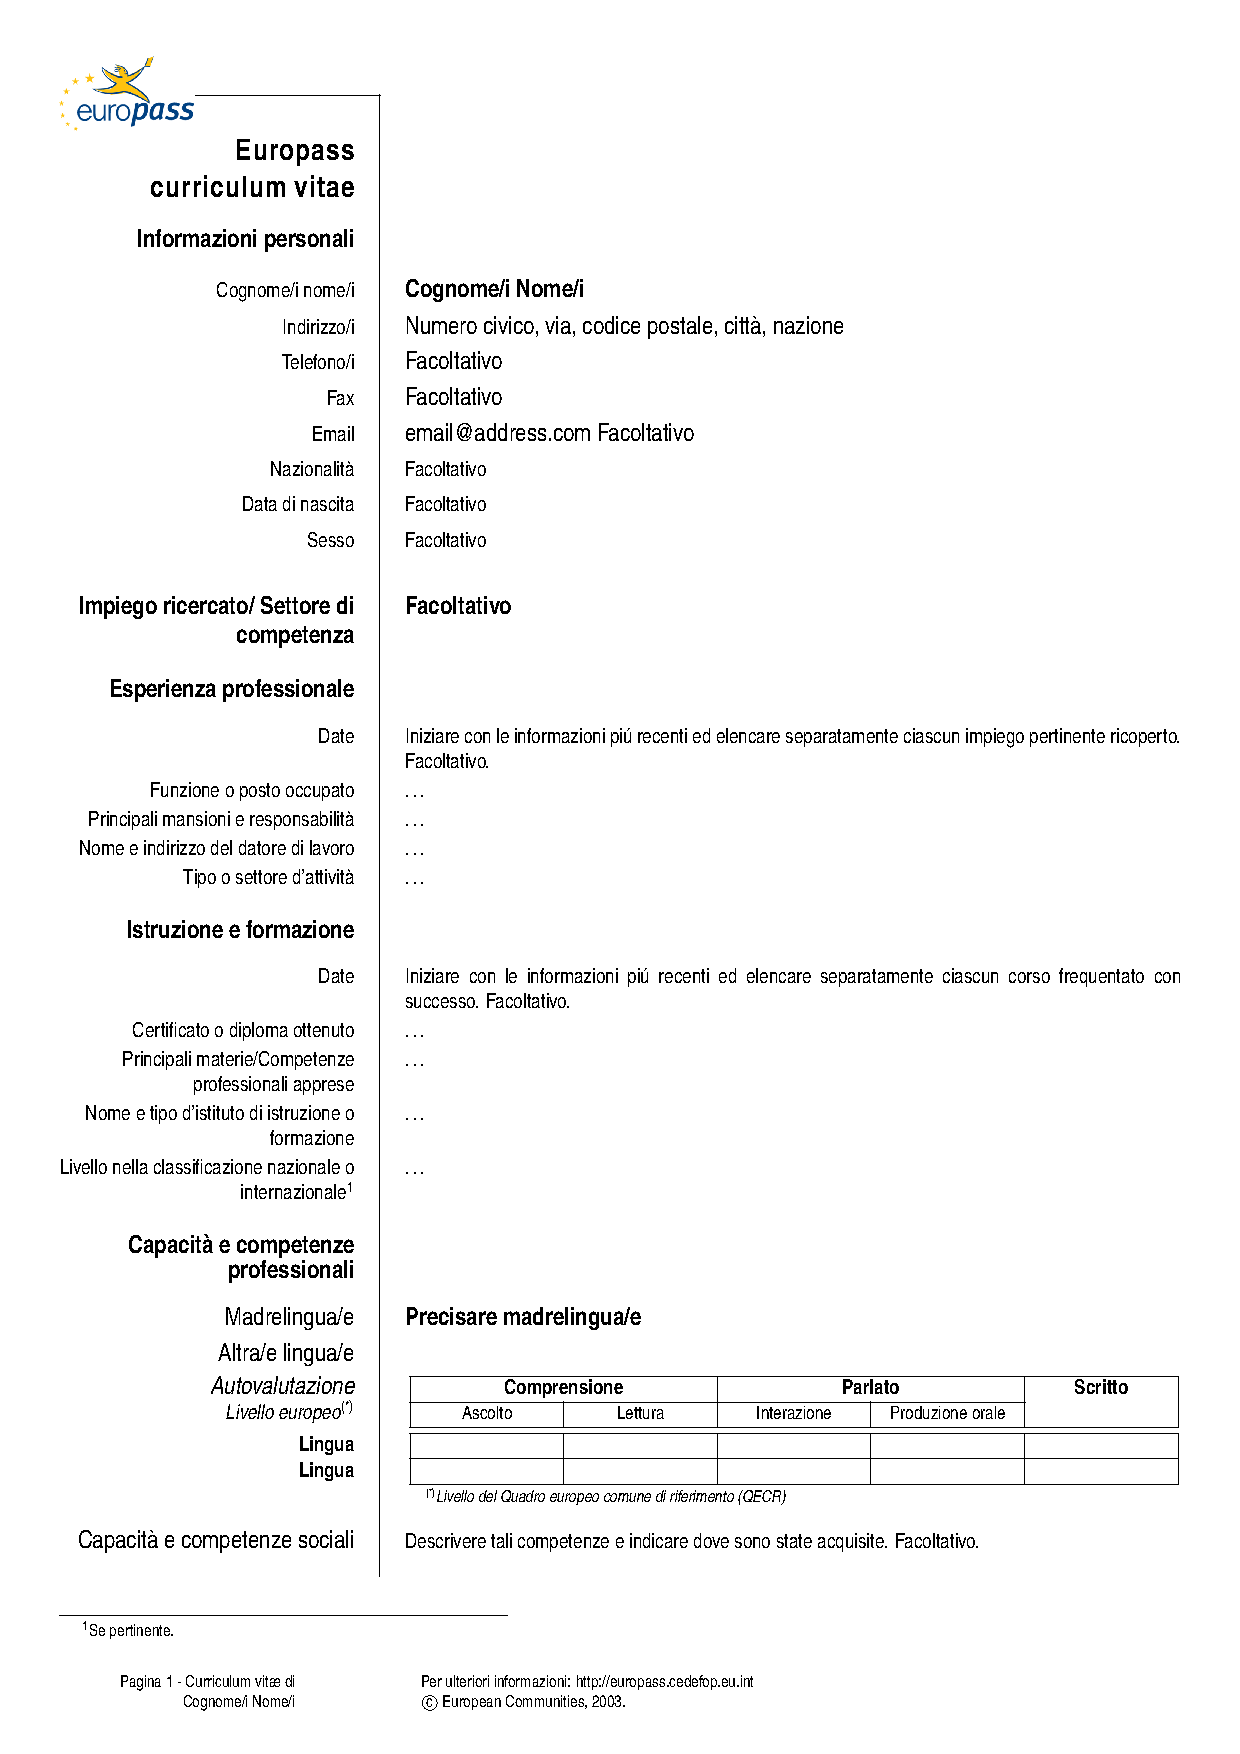
\includegraphics[height=.75\textheight]{europecv1}}
		\end{column}
	\end{columns}
\end{frame}
%-----------------------------------------------------------
%--------------------------------------------------- SLIDE z
\begin{frame}
  \frametitle{\texttt{moderncv}}
	\begin{columns}[c]
		\begin{column}{0.6\linewidth}
			\begin{itemize}
			\item \textbf{Pro}
				\begin{itemize}
				\item Layout molto chiaro ed accattivante (in due versioni, \Lopt{casual} e \Lopt{classic})
				\item Molto flessibile
				\item \emph{Template} chiari e ricchi di commenti
				\item Permette di redigere la lettera di presentazione
				\end{itemize}
			\end{itemize}
			\begin{block}{Quindi\dots}
			\`E una delle \textbf{migliori soluzioni} attualmente disponibili per realizzare un curriculum in \LaTeX.
			\end{block}
		\end{column}
		\begin{column}{0.4\linewidth}
			\centering
			\fbox{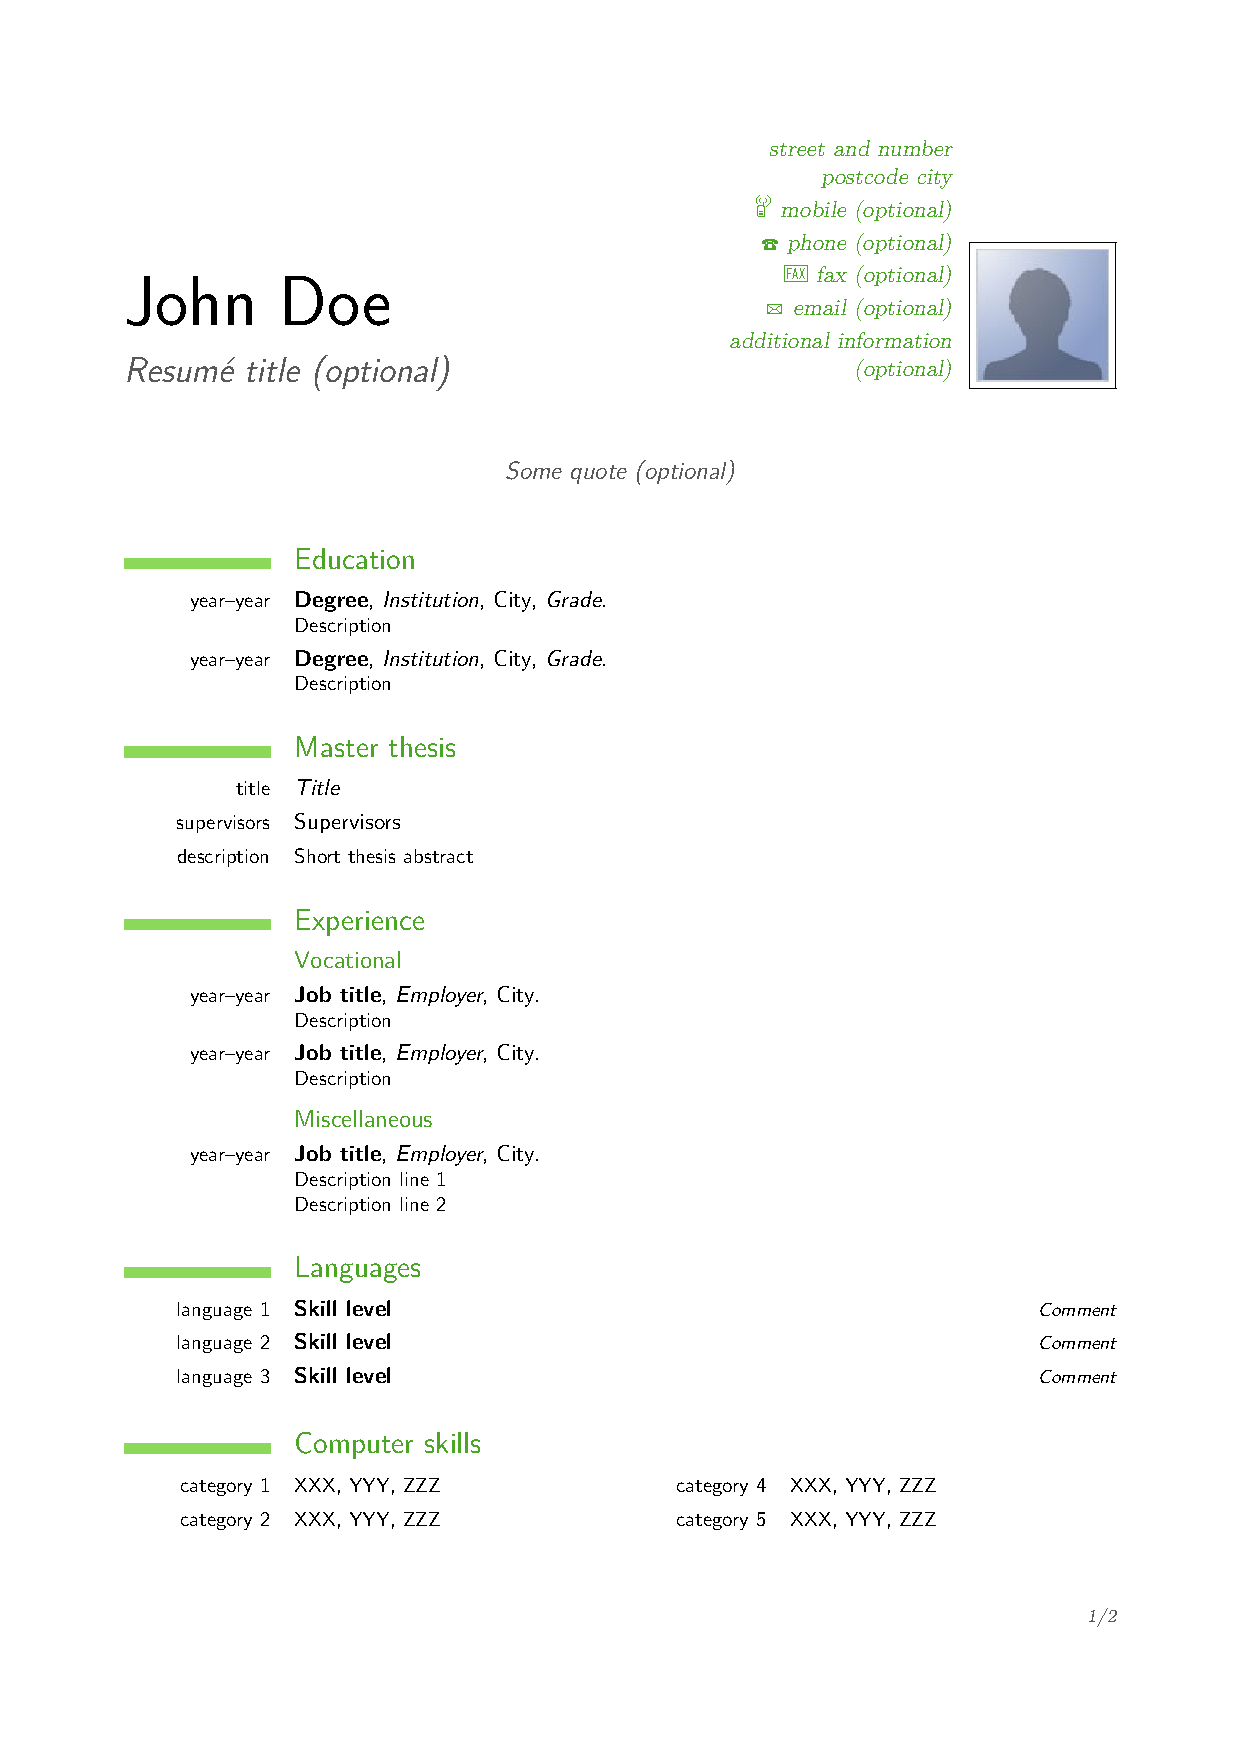
\includegraphics[height=.75\textheight]{moderncv}}
		\end{column}
	\end{columns}
\end{frame}
%-----------------------------------------------------------
%---------------------------------------------- SUBSECTION -
\subsection{Sintassi di base}
%-----------------------------------------------------------
%--------------------------------------------------- SLIDE -
\begin{frame}
  \frametitle{Il modello di un documento (\texttt{europecv})}
	\begin{LaTeXcode}
		\\documentclass\{\alert{europecv}\}\n
	  \onslide<2->
		\\usepackage\{<nome-package>\}\n
	  \onslide<3->
		\alert{\\ecvfirstname\{}<nome>\alert{\}}\n
		\alert{\\ecvlastname\{}<cognonome>\alert{\}}\n
		\hspace*{10ex}\vdots\n
	  \smallskip
	  \onslide<4->
		\\begin\{document\}\n
	  \onslide<5->
		\\selectlanguage\{italian\}\n
	  \onslide<6->
		\hspace*{5ex}\\begin\{\alert{europecv}\}\n
		\hspace*{15ex}\vdots\n
		\hspace*{5ex}\\end\{\alert{europecv}\}\n
	  \onslide<4->
		\smallskip
		\\end\{document\}
	\end{LaTeXcode}
\end{frame}
%-----------------------------------------------------------
%--------------------------------------------------- SLIDE -
\begin{frame}
  \frametitle{Il modello di un documento (\texttt{europecv})}
	\begin{LaTeXcode}
		\\begin\{europecv\}\n
	  \onslide<2->
		\hspace*{2ex}\alert{\\ecvsection\{}Esperienze lavorative\alert{\}}\n
	  \onslide<3->
		\hspace*{5ex}\alert{\\ecvitem\{}Data\alert{\}\{}Ottobre 2000 in poi\alert{\}}\n
		\hspace*{5ex}\alert{\\ecvitem\{}Azienda\alert{\}\{}Scuola Inferiore San Gianna\alert{\}}\n

	  \smallskip
	  \onslide<4->
		\hspace*{2ex}\\ecvsection\{Istruzione e Formazione\}\n
		\hspace*{5ex}\\ecvitem\{Data\}\{31 Febbraio 2005\}\n
		\hspace*{5ex}\\ecvitem\{Qualifica\}\{Laurea Elementare\}\n
		\hspace*{15ex}\vdots\n
		
	  \smallskip
	  \onslide<1->
		\smallskip
		\\end\{europecv\}
	\end{LaTeXcode}
\end{frame}
%-----------------------------------------------------------
%--------------------------------------------------- SLIDE -
\begin{frame}
  \frametitle{Un esempio vale pi\`u di mille parole}
	\begin{center}
		\alert{\texttt{esempio\_2\_9.tex}}
	\end{center}
\end{frame}
%-----------------------------------------------------------
%--------------------------------------------------- SLIDE -
\begin{frame}
  \frametitle{Il modello di un documento (\texttt{moderncv})}
	\begin{LaTeXcode}
		\\documentclass\{\alert{moderncv}\}\n
	  \onslide<2->
		\alert{\\moderncvtheme[blue]\{casual\}}\n
	  \onslide<3->
		\alert{\\firstname\{}<nome>\alert{\}}\n
		\alert{\\familyname\{}<cognome>\alert{\}}\n
		\\title\{\}\n
		\\address\{\alert{<strada>}\}\{\alert{<cap>}\}\n
		\\mobile\{\}\n
		\hspace*{10ex}\vdots\n
	  \smallskip
	  \onslide<4->
		\\begin\{document\}\n
		\smallskip
		\hspace*{10ex}\vdots\n
		\smallskip
		\\end\{document\}
	\end{LaTeXcode}
\end{frame}
%-----------------------------------------------------------
%--------------------------------------------------- SLIDE -
\begin{frame}
  \frametitle{Il modello di un documento (\texttt{moderncv})}
	\begin{LaTeXcode}
		\\begin\{document\}\n
	  \onslide<2->
		\alert{\\maketitle}\n
	  \onslide<3->
		\hspace*{2ex}\alert{\\section\{}Educazione\alert{\}}\n
		\hspace*{2ex}\alert{\\cventry\{}anno\alert{\}\{}laurea\alert{\}\{}istituzione\alert{\}\{}città\alert{\}}\n
		\hspace*{10ex}\alert{\{}grado\alert{\}\{}descrizione\alert{\}}\n
	  \smallskip
	  \onslide<4->
		\hspace*{2ex}\\section\{Diseducazione\}\n
		\hspace*{2ex}\\cvline\{Corso di Teppismo\}\{36 Febbraio 2005\}\n
		\hspace*{15ex}\vdots\n
	  \smallskip
	  \onslide<1->
		\smallskip
		\\end\{document\}

	\end{LaTeXcode}
\end{frame}
%-----------------------------------------------------------
%--------------------------------------------------- SLIDE -
\begin{frame}
  \frametitle{Un esempio vale pi\`u di mille parole}
	\begin{center}
		\alert{\texttt{esempio\_2\_10.tex}}
	\end{center}
\end{frame}
%-----------------------------------------------------------
%--------------------------------------------------- SLIDE -
\begin{frame}
  \frametitle{E anche per oggi abbiamo finito\dots}
	\begin{center}
	  \huge
		Grazie e alla prossima lezione
	\end{center}
  \medskip
	\begin{block}{Cosa impareremo la prossima volta}
		\begin{itemize}
			\item \textbf{oggetti flottanti} 
			\item come realizzare le \textbf{tabelle} 
			\item \textbf{formule matematiche} allo stato dell'arte
			\item gestire i \textbf{riferimenti bibliografici} in modo semplice ed efficiente
		\end{itemize}
	\end{block}
\end{frame}
%-----------------------------------------------------------
%----------------------------------------------------- END -

\end{document}
